\documentclass[10pt,a4paper]{article}
\usepackage[utf8]{inputenc}
\usepackage{amsmath}
\usepackage{amsfonts}
\usepackage{amssymb}
\usepackage{graphicx}
\usepackage{booktabs}
\usepackage{subfig}
\author{Marcello Nieddu}
\begin{document}
\section{Abstract}
The aim of this exercise is to build an AB version of the models of chapter 3 (SIM model) and 4 (PC model) of \cite{godley2006monetary}.

\section{SIM model}
Assumptions are
\begin{enumerate}
\item closed economy
\item agents other than government can be conceptually divided in Households, when they receive income and consume and accumulate assets, and Production when they sell service and pay out wages.
\item production undertaken by providers of services; they have no capital and no intermediate production costs
\item there are no banks, no firms, no profit
\item there are not interests payment
\item there is only government money
\end{enumerate}
\subsection{non formal model}
Target system: imaginary population where economy is simplified.

There is a government that creates money. Citizens can sell and pay wages, recive wages, pay taxes, consume and deposit money. These activities in the book are ideally subdivided in two: household activities and producer or production firm owner activities.



\subsection{formal model}
Since we  want an ABM of this target system we have to explicitly represent entities and their relations in our model.

Following Galan et al. \cite{galan2009errors}:

\begin{quote}
Modelling is the process of building an abstraction of a system for a specific purpose. Thus, in essence, what distinguishes one modelling paradigm from another is precisely the way we construct that abstraction from the observed system. [...] agent-based modelling is a modelling paradigm with the defining characteristic that entities within the target system to be modelled and the interactions between them are explicitly and individually represented in the model (see Figure 1). This is in contrast to other models where some entities are represented via average properties or via single representative agents.
\end{quote}

So every agent can act both as household or as producer. Agents are inserted in networks that represent interactions and relations among agents. In our model relation between agents are encoded in two static (exogenous) directed networks, one for the working relations, the other for selling relations. In a more realistic model networks co-evolve with agents. 


\subsection{executable model}
Two class of agents, government and Eagent (economic agent).

\begin{table}[h]
\centering
\begin{tabular}{lc}
\toprule
\textbf{Government}  & \\
\midrule
Data member & \\
\midrule
1 & G \\
2 & $\theta$ \\
3 &cash \\
4 & TFM \\
\midrule
Methods & \\
\midrule
1 & consume \\
2 & receiveTaxes\\
3 & createList\\
4 & write on DB\\
5 & resetTFM\\
\bottomrule
\end{tabular}
\caption{Government class}
\label{GovClass}
\end{table}

Table \ref{GovClass} shows Government class. $G$ and $\theta$ are external parameters of the (formal) model. \emph{cash} is the only stock of Government. \emph{TFM} is a Transaction Flow Matrix object that the government use to accounting its activities; this is a data member introduced to the needs of executable model. The first three methods are due to the formal model, the last two belong to the executable model: in order to simplify data acquisition we introduce the hypothesis that every agent takes track of its economic activity through a transaction flow matrix.

Every time 





\begin{table}[h]
\centering
\begin{tabular}{lc}
\toprule
\textbf{Eagent}  & \\
\midrule
Data member & \\
\midrule
1 & $\alpha_1$ \\
2 & $\alpha_2$ \\
3 &cash \\
4 & householdTFM \\
5 & producerTFM \\
6 & workersList \\
7 & sellerList\\
8 & income\\
9 & sold\\
\midrule
Methods & \\
\midrule
1 & receiveWage \\
2 & payTaxes\\
3 & consume \\
4 & consumeFromCash\\
5 & deposit\\
6 & sell\\
7 & payWages\\
8 & createList\\
9 & write on DB\\
10 & resetTFM\\
\bottomrule
\end{tabular}
\caption{Economic agent class}
\label{EagentClass}
\end{table}
In table \ref{EagentClass} it is shown the Eagent class. As for the government there are variables whose existence is due to executable model needs. So the first 3 data members and the first seven methods pertain to the theoretical model, the others to the executable one.


VERY IMPORTANT: agents consume until their income is lower than $0.00001$. This is the way we implement the fact that in the tematitian model agents consume (and deposit) all their wages. This introduce finite time effect that may led the model to slightly different states from those observed in the theoretical model.
\subsection{Results}

First we reproduce the results shown in table 3.4 of \cite{godley2006monetary}. Here $\alpha_1 = 0.6$, $\alpha_2 = 0.4$, the tax rate $\theta = 0.2$. Every reference period is $30$ iterations long, and the system has been observed for $100$ of periods.

\begin{table}[h]
\centering
\begin{tabular}{llcrr}
\toprule
Stock & 0 & 1 & 2 & 99\\
\midrule
G & 20 & 20 & 20 & 20\\
Y & 38.461392 & 47.928837 &	55.939828 &	1.000000e+02 \\
T &	7.692278 &	9.585767 &	11.187966 &	2.000000e+01 \\
YD & 30,769113 &	38,343070 &	44,751862 &	79,999997 \\
C &	18.461392 & 27.928837 &	35.939828 &	8.000000e+01 \\
$\Delta H$ &	12.307722 &	10.414233 &	8.812034 &	8.084872e-07 \\
\bottomrule
\end{tabular} 
\caption{Here $\alpha_1 = 0.6$, $\alpha_2 = 0.4$, the tax rate $\theta = 0.2$. Every reference period is $30$ iterations long, and the system has been observed for $100$ of periods.}
\end{table}

Then we explore model behavior to changing parameters.



Then we exploit the proprieties of ABM to analyze the distribution of wealth among agents. In the figure \ref{WealthDistribution} are shown the histograms of wealth distribution. The first is relative to homogeneous agents, all having the same values of the paramameters $\alpha_1$ and $\alpha_2$. The second refers to heterogeneous agents: the values of $\alpha_1$ 
are picked at random from a uniform distribution in the interval $[0,1]$.
\begin{figure}[h]
\centering
\subfloat[][Homogeneous agents]{
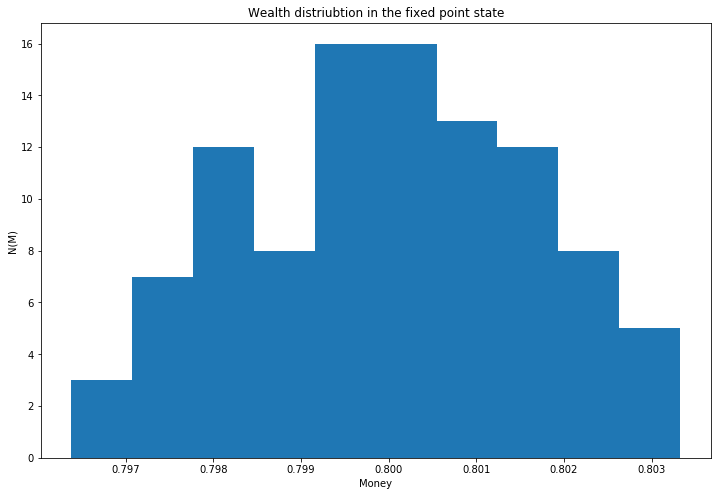
\includegraphics[scale=0.2]{Wealth100}}\\
\subfloat[][Heterogeneous agents]{
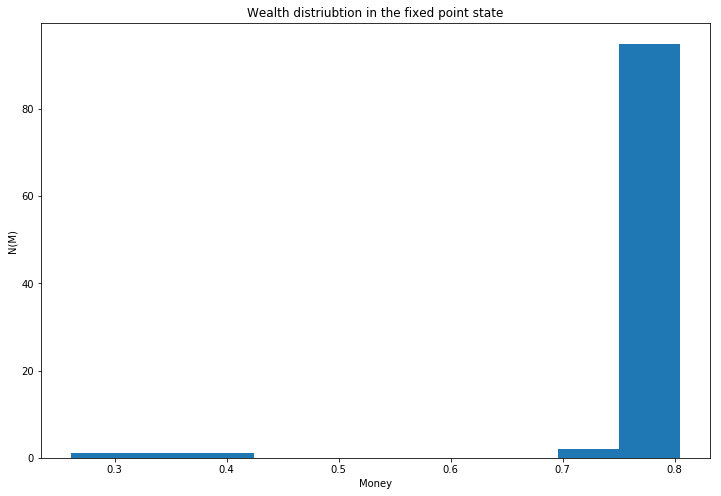
\includegraphics[scale=0.2]{WealthUniform}}
\caption{Wealth distribution}
\label{WealthDistribution}
\end{figure}


What happen if we change the structure of interactions graph?

The steady state (which is a stationary state) is characterized by the relation
\begin{equation}
Y^* = \frac{G}{\theta}
\end{equation}
Our purpose is to check if this equation still holds when we deal with heterogeneous agents (for instance: heterogeneous in their consumption function)


\begin{table}[h]
\centering
\begin{tabular}{lrrrr}
\toprule
Period &         0  &         1  &         2  &          99 \\
\midrule
Y &  47.284729 &  60.659901 &  71.388738 &  116.192949 \\
C  & 27.284729 & 40.659901 & 51.388738 &  96.192949 \\
H  &  10.543054 &   7.868020 &   5.722252 &   3.238590 \\
T  &  9.456946 & 12.131980 & 14.277748 &  23.238590 \\
\bottomrule
\end{tabular}
\caption{Final results with 10 agents in a E-R graph, with heterogeneous consumption function}
\end{table}

\begin{table}[h]
\centering
\begin{tabular}{lrrr}
\toprule
Sector &  Government &   Household &    Producer \\
\midrule
C  &    0.000000 &  -82.268884 &   82.268884 \\
G  &  -20.000000 &    0.000000 &   20.000000 \\
WB &    0.000000 &  102.268884 & -102.268884 \\
T  &   20.453777 &  -20.453777 &    0.000000 \\
$\Delta H$  &    0.453777 &   -0.453777 &    0.000000 \\
\bottomrule
\end{tabular}
\caption{asymptotic TF matrix. 100 of agents, with heterogeneous consumption function and with a E-R graph to represent working relation}
\end{table}

\begin{figure}[h]
\centering
\subfloat[][Homogeneous agents in a complete graph]{
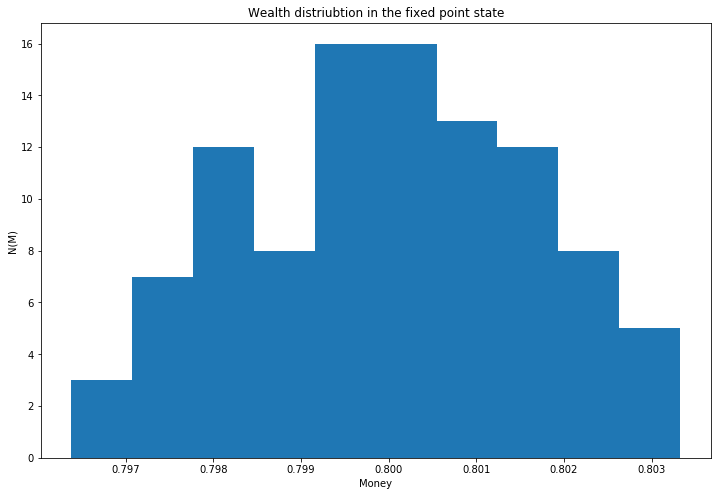
\includegraphics[scale=0.2]{Wealth100}}\\
\subfloat[][Heterogeneous agents in a Erdos-Renyi graph]{
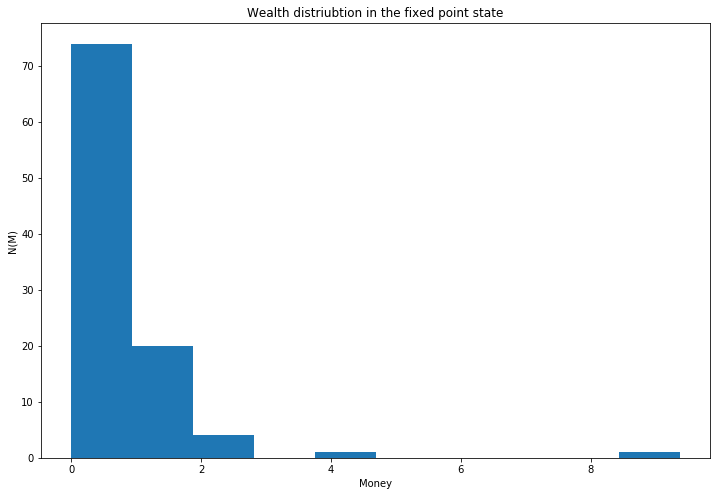
\includegraphics[scale=0.2]{WealthHetER}}
\caption{Wealth distribution}
\label{WealthDistribution}
\end{figure}


\bibliography{./Bibliografia}
\bibliographystyle{plain}
\end{document}